

\section{Problem 2}
\label{part2}
\begin{verbatim}
Which 5 users are most correlated to the substitute you? Which 5 users are least correlated 
(i.e., negative correlation)?


\end{verbatim}

\subsection{Solution}
\begin{enumerate}
\item In this question I need to find out 5 users who are most and least correlated to my substitute.
\item For doing this I used some function from recommendations.py as reference taken from a book called ``Programming Collective Intelligence.''
\item I used u.data file and sent it as input to my program to get the solution. The program can be found in listing\ref{lst:q2-1}.
\item For doing this I need to find the sim pearson's coefficient which for each user.
\item If the coefficient for each user is 1 or nearer to 1, then that user is most correlated to my substitute and if the coefficient is negative then that user is least coefficient to my substitute.
\item I found the top 5 most correlated users and bottom 5 least correlated users which can be seen in fig\ref{Samplet2}.
\item First column represent the value of coefficient followed by user-id.
\end{enumerate}
\newpage

\subsection{Code Listing}

\lstinputlisting[language=Python,breaklines = true,frame=single,caption={Python Code for getting finding gender of each follower}, label=lst:q2-1,captionpos=b,numbers=left,showspaces=false,showstringspaces=false,basicstyle=\footnotesize]{mov_2.py}
\newpage

\subsection{Inputs}
\subsubsection{Sample u.data file}
\begin{figure}[ht]    
    \begin{center}
        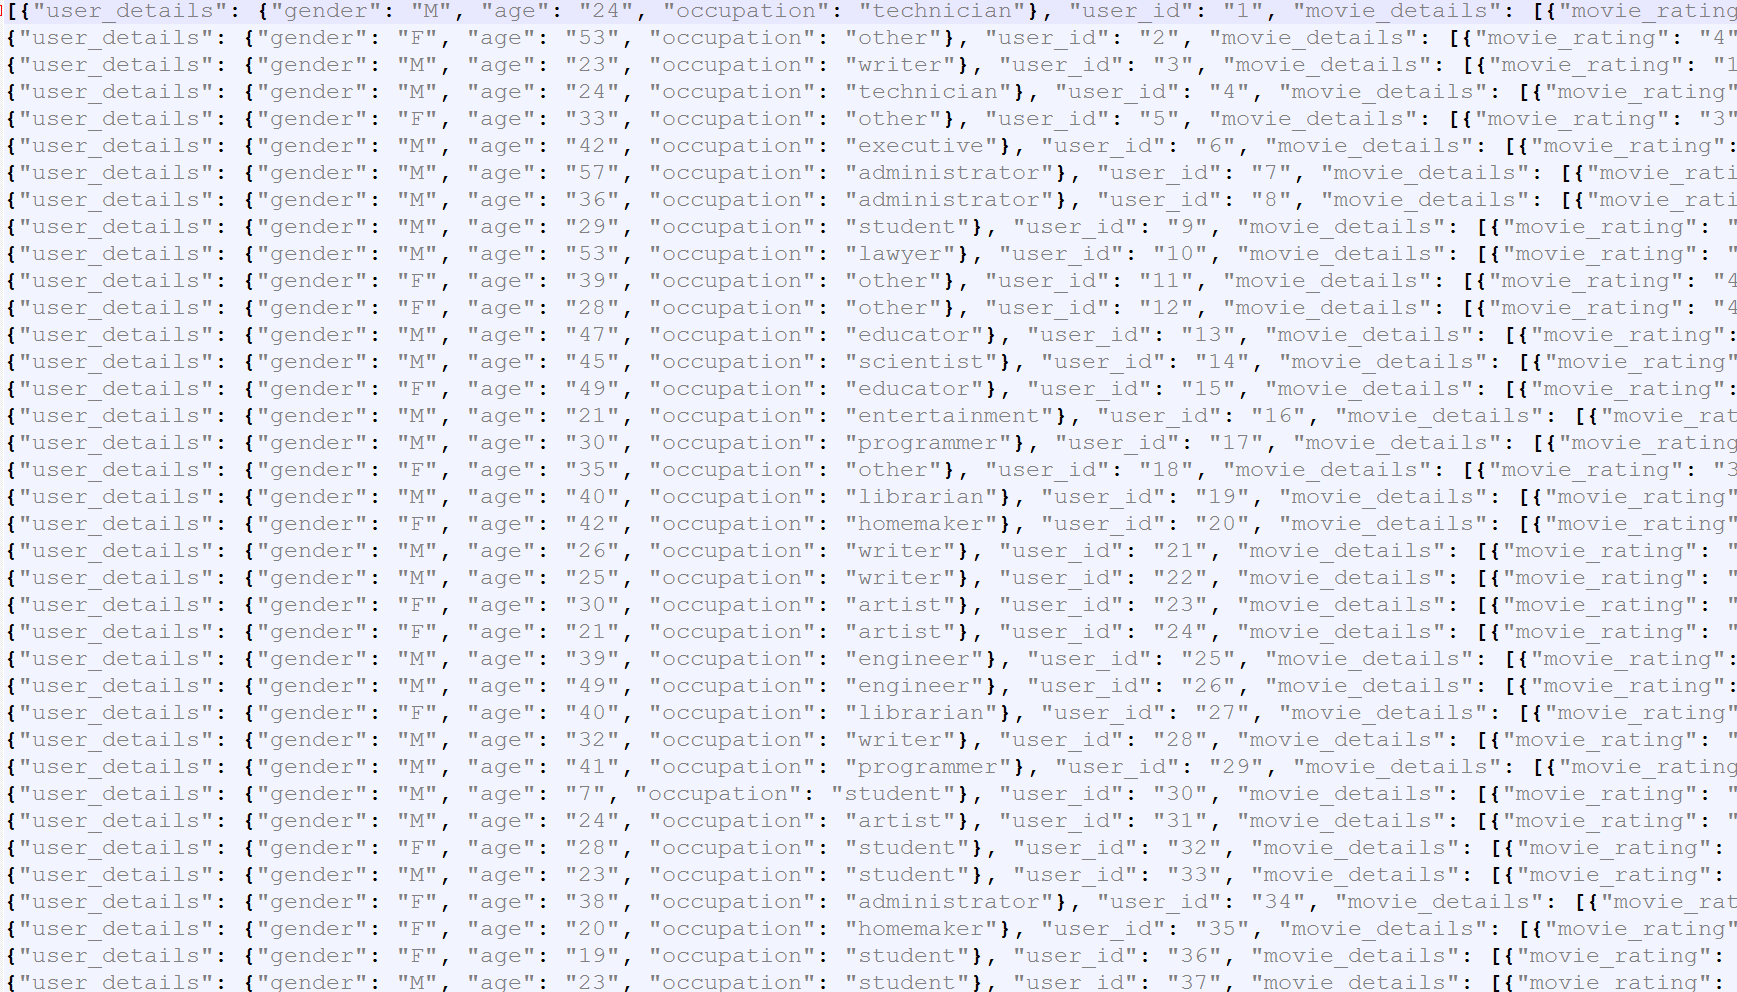
\includegraphics[scale=0.4]{sample_udata.png}
        \caption{Sample list of users and their rating for each movie}
        \label{Samplet1}
    \end{center}
\end{figure}
\newpage

\subsection{Output}

\subsubsection{output file}
\begin{figure}[ht]    
    \begin{center}
        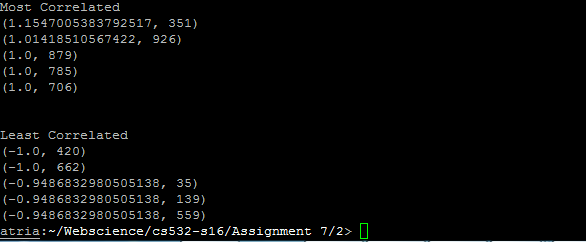
\includegraphics[scale=1.0]{mostandleastcorrelated.png}
        \caption{File shows 5 users with their user id's on right side who are most correlated and least correlated to my substitute}
        \label{Samplet2}
    \end{center}
\end{figure}
\newpage
